%********************************************%
%*       Generated from PreTeXt source      *%
%*       on 2022-01-13T09:49:29-06:00       *%
%*   A recent stable commit (2020-08-09):   *%
%* 98f21740783f166a773df4dc83cab5293ab63a4a *%
%*                                          *%
%*         https://pretextbook.org          *%
%*                                          *%
%********************************************%
%% We elect to always write snapshot output into <job>.dep file
\RequirePackage{snapshot}
\documentclass[oneside,10pt,]{book}
%% Custom Preamble Entries, early (use latex.preamble.early)
%% Default LaTeX packages
%%   1.  always employed (or nearly so) for some purpose, or
%%   2.  a stylewriter may assume their presence
\usepackage{geometry}
%% Some aspects of the preamble are conditional,
%% the LaTeX engine is one such determinant
\usepackage{ifthen}
%% etoolbox has a variety of modern conveniences
\usepackage{etoolbox}
\usepackage{ifxetex,ifluatex}
%% Raster graphics inclusion
\usepackage{graphicx}
%% Color support, xcolor package
%% Always loaded, for: add/delete text, author tools
%% Here, since tcolorbox loads tikz, and tikz loads xcolor
\PassOptionsToPackage{usenames,dvipsnames,svgnames,table}{xcolor}
\usepackage{xcolor}
%% begin: defined colors, via xcolor package, for styling
%% end: defined colors, via xcolor package, for styling
%% Colored boxes, and much more, though mostly styling
%% skins library provides "enhanced" skin, employing tikzpicture
%% boxes may be configured as "breakable" or "unbreakable"
%% "raster" controls grids of boxes, aka side-by-side
\usepackage{tcolorbox}
\tcbuselibrary{skins}
\tcbuselibrary{breakable}
\tcbuselibrary{raster}
%% We load some "stock" tcolorbox styles that we use a lot
%% Placement here is provisional, there will be some color work also
%% First, black on white, no border, transparent, but no assumption about titles
\tcbset{ bwminimalstyle/.style={size=minimal, boxrule=-0.3pt, frame empty,
colback=white, colbacktitle=white, coltitle=black, opacityfill=0.0} }
%% Second, bold title, run-in to text/paragraph/heading
%% Space afterwards will be controlled by environment,
%% independent of constructions of the tcb title
%% Places \blocktitlefont onto many block titles
\tcbset{ runintitlestyle/.style={fonttitle=\blocktitlefont\upshape\bfseries, attach title to upper} }
%% Spacing prior to each exercise, anywhere
\tcbset{ exercisespacingstyle/.style={before skip={1.5ex plus 0.5ex}} }
%% Spacing prior to each block
\tcbset{ blockspacingstyle/.style={before skip={2.0ex plus 0.5ex}} }
%% xparse allows the construction of more robust commands,
%% this is a necessity for isolating styling and behavior
%% The tcolorbox library of the same name loads the base library
\tcbuselibrary{xparse}
%% The tcolorbox library loads TikZ, its calc package is generally useful,
%% and is necessary for some smaller documents that use partial tcolor boxes
%% See:  https://github.com/rbeezer/mathbook/issues/1624
\usetikzlibrary{calc}
%% Hyperref should be here, but likes to be loaded late
%%
%% Inline math delimiters, \(, \), need to be robust
%% 2016-01-31:  latexrelease.sty  supersedes  fixltx2e.sty
%% If  latexrelease.sty  exists, bugfix is in kernel
%% If not, bugfix is in  fixltx2e.sty
%% See:  https://tug.org/TUGboat/tb36-3/tb114ltnews22.pdf
%% and read "Fewer fragile commands" in distribution's  latexchanges.pdf
\IfFileExists{latexrelease.sty}{}{\usepackage{fixltx2e}}
%% Footnote counters and part/chapter counters are manipulated
%% April 2018:  chngcntr  commands now integrated into the kernel,
%% but circa 2018/2019 the package would still try to redefine them,
%% so we need to do the work of loading conditionally for old kernels.
%% From version 1.1a,  chngcntr  should detect defintions made by LaTeX kernel.
\ifdefined\counterwithin
\else
    \usepackage{chngcntr}
\fi
%% Text height identically 9 inches, text width varies on point size
%% See Bringhurst 2.1.1 on measure for recommendations
%% 75 characters per line (count spaces, punctuation) is target
%% which is the upper limit of Bringhurst's recommendations
\geometry{letterpaper,total={340pt,9.0in}}
%% Custom Page Layout Adjustments (use latex.geometry)
%% This LaTeX file may be compiled with pdflatex, xelatex, or lualatex executables
%% LuaTeX is not explicitly supported, but we do accept additions from knowledgeable users
%% The conditional below provides  pdflatex  specific configuration last
%% begin: engine-specific capabilities
\ifthenelse{\boolean{xetex} \or \boolean{luatex}}{%
%% begin: xelatex and lualatex-specific default configuration
\ifxetex\usepackage{xltxtra}\fi
%% realscripts is the only part of xltxtra relevant to lualatex 
\ifluatex\usepackage{realscripts}\fi
%% end:   xelatex and lualatex-specific default configuration
}{
%% begin: pdflatex-specific default configuration
%% We assume a PreTeXt XML source file may have Unicode characters
%% and so we ask LaTeX to parse a UTF-8 encoded file
%% This may work well for accented characters in Western language,
%% but not with Greek, Asian languages, etc.
%% When this is not good enough, switch to the  xelatex  engine
%% where Unicode is better supported (encouraged, even)
\usepackage[utf8]{inputenc}
%% end: pdflatex-specific default configuration
}
%% end:   engine-specific capabilities
%%
%% Fonts.  Conditional on LaTex engine employed.
%% Default Text Font: The Latin Modern fonts are
%% "enhanced versions of the [original TeX] Computer Modern fonts."
%% We use them as the default text font for PreTeXt output.
%% Default Monospace font: Inconsolata (aka zi4)
%% Sponsored by TUG: http://levien.com/type/myfonts/inconsolata.html
%% Loaded for documents with intentional objects requiring monospace
%% See package documentation for excellent instructions
%% fontspec will work universally if we use filename to locate OTF files
%% Loads the "upquote" package as needed, so we don't have to
%% Upright quotes might come from the  textcomp  package, which we also use
%% We employ the shapely \ell to match Google Font version
%% pdflatex: "varl" package option produces shapely \ell
%% pdflatex: "var0" package option produces plain zero (not used)
%% pdflatex: "varqu" package option produces best upright quotes
%% xelatex,lualatex: add OTF StylisticSet 1 for shapely \ell
%% xelatex,lualatex: add OTF StylisticSet 2 for plain zero (not used)
%% xelatex,lualatex: add OTF StylisticSet 3 for upright quotes
%%
%% Automatic Font Control
%% Portions of a document, are, or may, be affected by defined commands
%% These are perhaps more flexible when using  xelatex  rather than  pdflatex
%% The following definitions are meant to be re-defined in a style, using \renewcommand
%% They are scoped when employed (in a TeX group), and so should not be defined with an argument
\newcommand{\divisionfont}{\relax}
\newcommand{\blocktitlefont}{\relax}
\newcommand{\contentsfont}{\relax}
\newcommand{\pagefont}{\relax}
\newcommand{\tabularfont}{\relax}
\newcommand{\xreffont}{\relax}
\newcommand{\titlepagefont}{\relax}
%%
\ifthenelse{\boolean{xetex} \or \boolean{luatex}}{%
%% begin: font setup and configuration for use with xelatex
%% Generally, xelatex is necessary for non-Western fonts
%% fontspec package provides extensive control of system fonts,
%% meaning *.otf (OpenType), and apparently *.ttf (TrueType)
%% that live *outside* your TeX/MF tree, and are controlled by your *system*
%% (it is possible that a TeX distribution will place fonts in a system location)
%%
%% The fontspec package is the best vehicle for using different fonts in  xelatex
%% So we load it always, no matter what a publisher or style might want
%%
\usepackage{fontspec}
%%
%% begin: xelatex main font ("font-xelatex-main" template)
%% Latin Modern Roman is the default font for xelatex and so is loaded with a TU encoding
%% *in the format* so we can't touch it, only perhaps adjust it later
%% in one of two ways (then known by NFSS names such as "lmr")
%% (1) via NFSS with font family names such as "lmr" and "lmss"
%% (2) via fontspec with commands like \setmainfont{Latin Modern Roman}
%% The latter requires the font to be known at the system-level by its font name,
%% but will give access to OTF font features through optional arguments
%% https://tex.stackexchange.com/questions/470008/
%% where-and-how-does-fontspec-sty-specify-the-default-font-latin-modern-roman
%% http://tex.stackexchange.com/questions/115321
%% /how-to-optimize-latin-modern-font-with-xelatex
%%
%% end:   xelatex main font ("font-xelatex-main" template)
%% begin: xelatex mono font ("font-xelatex-mono" template)
%% (conditional on non-trivial uses being present in source)
\IfFontExistsTF{Inconsolatazi4-Regular.otf}{}{\GenericError{}{The font "Inconsolatazi4-Regular.otf" requested by PreTeXt output is not available.  Either a file cannot be located in default locations via a filename, or a font is not known by its name as part of your system.}{Consult the PreTeXt Guide for help with LaTeX fonts.}{}}
\IfFontExistsTF{Inconsolatazi4-Bold.otf}{}{\GenericError{}{The font "Inconsolatazi4-Bold.otf" requested by PreTeXt output is not available.  Either a file cannot be located in default locations via a filename, or a font is not known by its name as part of your system.}{Consult the PreTeXt Guide for help with LaTeX fonts.}{}}
\usepackage{zi4}
\setmonofont[BoldFont=Inconsolatazi4-Bold.otf,StylisticSet={1,3}]{Inconsolatazi4-Regular.otf}
%% end:   xelatex mono font ("font-xelatex-mono" template)
%% begin: xelatex font adjustments ("font-xelatex-style" template)
%% end:   xelatex font adjustments ("font-xelatex-style" template)
%%
%% Extensive support for other languages
\usepackage{polyglossia}
%% Set main/default language based on pretext/@xml:lang value
%% document language code is "en-US", US English
%% usmax variant has extra hypenation
\setmainlanguage[variant=usmax]{english}
%% Enable secondary languages based on discovery of @xml:lang values
%% Enable fonts/scripts based on discovery of @xml:lang values
%% Western languages should be ably covered by Latin Modern Roman
%% end:   font setup and configuration for use with xelatex
}{%
%% begin: font setup and configuration for use with pdflatex
%% begin: pdflatex main font ("font-pdflatex-main" template)
\usepackage{lmodern}
\usepackage[T1]{fontenc}
%% end:   pdflatex main font ("font-pdflatex-main" template)
%% begin: pdflatex mono font ("font-pdflatex-mono" template)
%% (conditional on non-trivial uses being present in source)
\usepackage[varqu,varl]{inconsolata}
%% end:   pdflatex mono font ("font-pdflatex-mono" template)
%% begin: pdflatex font adjustments ("font-pdflatex-style" template)
%% end:   pdflatex font adjustments ("font-pdflatex-style" template)
%% end:   font setup and configuration for use with pdflatex
}
%% Micromanage spacing, etc.  The named "microtype-options"
%% template may be employed to fine-tune package behavior
\usepackage{microtype}
%% Symbols, align environment, commutative diagrams, bracket-matrix
\usepackage{amsmath}
\usepackage{amscd}
\usepackage{amssymb}
%% allow page breaks within display mathematics anywhere
%% level 4 is maximally permissive
%% this is exactly the opposite of AMSmath package philosophy
%% there are per-display, and per-equation options to control this
%% split, aligned, gathered, and alignedat are not affected
\allowdisplaybreaks[4]
%% allow more columns to a matrix
%% can make this even bigger by overriding with  latex.preamble.late  processing option
\setcounter{MaxMatrixCols}{30}
%%
%%
%% Division Titles, and Page Headers/Footers
%% titlesec package, loading "titleps" package cooperatively
%% See code comments about the necessity and purpose of "explicit" option.
%% The "newparttoc" option causes a consistent entry for parts in the ToC 
%% file, but it is only effective if there is a \titleformat for \part.
%% "pagestyles" loads the  titleps  package cooperatively.
\usepackage[explicit, newparttoc, pagestyles]{titlesec}
%% The companion titletoc package for the ToC.
\usepackage{titletoc}
%% Fixes a bug with transition from chapters to appendices in a "book"
%% See generating XSL code for more details about necessity
\newtitlemark{\chaptertitlename}
%% begin: customizations of page styles via the modal "titleps-style" template
%% Designed to use commands from the LaTeX "titleps" package
%% Plain pages should have the same font for page numbers
\renewpagestyle{plain}{%
\setfoot{}{\pagefont\thepage}{}%
}%
%% Single pages as in default LaTeX
\renewpagestyle{headings}{%
\sethead{\pagefont\slshape\MakeUppercase{\ifthechapter{\chaptertitlename\space\thechapter.\space}{}\chaptertitle}}{}{\pagefont\thepage}%
}%
\pagestyle{headings}
%% end: customizations of page styles via the modal "titleps-style" template
%%
%% Create globally-available macros to be provided for style writers
%% These are redefined for each occurence of each division
\newcommand{\divisionnameptx}{\relax}%
\newcommand{\titleptx}{\relax}%
\newcommand{\subtitleptx}{\relax}%
\newcommand{\shortitleptx}{\relax}%
\newcommand{\authorsptx}{\relax}%
\newcommand{\epigraphptx}{\relax}%
%% Create environments for possible occurences of each division
%% Environment for a PTX "chapter" at the level of a LaTeX "chapter"
\NewDocumentEnvironment{chapterptx}{mmmmmm}
{%
\renewcommand{\divisionnameptx}{Chapter}%
\renewcommand{\titleptx}{#1}%
\renewcommand{\subtitleptx}{#2}%
\renewcommand{\shortitleptx}{#3}%
\renewcommand{\authorsptx}{#4}%
\renewcommand{\epigraphptx}{#5}%
\chapter[{#3}]{#1}%
\label{#6}%
}{}%
%% Environment for a PTX "section" at the level of a LaTeX "section"
\NewDocumentEnvironment{sectionptx}{mmmmmm}
{%
\renewcommand{\divisionnameptx}{Section}%
\renewcommand{\titleptx}{#1}%
\renewcommand{\subtitleptx}{#2}%
\renewcommand{\shortitleptx}{#3}%
\renewcommand{\authorsptx}{#4}%
\renewcommand{\epigraphptx}{#5}%
\section[{#3}]{#1}%
\label{#6}%
}{}%
%% Environment for a PTX "subsection" at the level of a LaTeX "subsection"
\NewDocumentEnvironment{subsectionptx}{mmmmmm}
{%
\renewcommand{\divisionnameptx}{Subsection}%
\renewcommand{\titleptx}{#1}%
\renewcommand{\subtitleptx}{#2}%
\renewcommand{\shortitleptx}{#3}%
\renewcommand{\authorsptx}{#4}%
\renewcommand{\epigraphptx}{#5}%
\subsection[{#3}]{#1}%
\label{#6}%
}{}%
%% Environment for a PTX "index" at the level of a LaTeX ""
\NewDocumentEnvironment{indexptx}{mmmmmm}
{%
\renewcommand{\divisionnameptx}{Index}%
\renewcommand{\titleptx}{#1}%
\renewcommand{\subtitleptx}{#2}%
\renewcommand{\shortitleptx}{#3}%
\renewcommand{\authorsptx}{#4}%
\renewcommand{\epigraphptx}{#5}%
\*{#1}%
\addcontentsline{toc}{}{#3}
\label{#6}%
}{}%
%% Environment for a PTX "appendix" at the level of a LaTeX "chapter"
\NewDocumentEnvironment{appendixptx}{mmmmmm}
{%
\renewcommand{\divisionnameptx}{Appendix}%
\renewcommand{\titleptx}{#1}%
\renewcommand{\subtitleptx}{#2}%
\renewcommand{\shortitleptx}{#3}%
\renewcommand{\authorsptx}{#4}%
\renewcommand{\epigraphptx}{#5}%
\chapter[{#3}]{#1}%
\label{#6}%
}{}%
%%
%% Styles for six traditional LaTeX divisions
\titleformat{\part}[display]
{\divisionfont\Huge\bfseries\centering}{\divisionnameptx\space\thepart}{30pt}{\Huge#1}
[{\Large\centering\authorsptx}]
\titleformat{\chapter}[display]
{\divisionfont\huge\bfseries}{\divisionnameptx\space\thechapter}{20pt}{\Huge#1}
[{\Large\authorsptx}]
\titleformat{name=\chapter,numberless}[display]
{\divisionfont\huge\bfseries}{}{0pt}{#1}
[{\Large\authorsptx}]
\titlespacing*{\chapter}{0pt}{50pt}{40pt}
\titleformat{\section}[hang]
{\divisionfont\Large\bfseries}{\thesection}{1ex}{#1}
[{\large\authorsptx}]
\titleformat{name=\section,numberless}[block]
{\divisionfont\Large\bfseries}{}{0pt}{#1}
[{\large\authorsptx}]
\titlespacing*{\section}{0pt}{3.5ex plus 1ex minus .2ex}{2.3ex plus .2ex}
\titleformat{\subsection}[hang]
{\divisionfont\large\bfseries}{\thesubsection}{1ex}{#1}
[{\normalsize\authorsptx}]
\titleformat{name=\subsection,numberless}[block]
{\divisionfont\large\bfseries}{}{0pt}{#1}
[{\normalsize\authorsptx}]
\titlespacing*{\subsection}{0pt}{3.25ex plus 1ex minus .2ex}{1.5ex plus .2ex}
\titleformat{\subsubsection}[hang]
{\divisionfont\normalsize\bfseries}{\thesubsubsection}{1em}{#1}
[{\small\authorsptx}]
\titleformat{name=\subsubsection,numberless}[block]
{\divisionfont\normalsize\bfseries}{}{0pt}{#1}
[{\normalsize\authorsptx}]
\titlespacing*{\subsubsection}{0pt}{3.25ex plus 1ex minus .2ex}{1.5ex plus .2ex}
\titleformat{\paragraph}[hang]
{\divisionfont\normalsize\bfseries}{\theparagraph}{1em}{#1}
[{\small\authorsptx}]
\titleformat{name=\paragraph,numberless}[block]
{\divisionfont\normalsize\bfseries}{}{0pt}{#1}
[{\normalsize\authorsptx}]
\titlespacing*{\paragraph}{0pt}{3.25ex plus 1ex minus .2ex}{1.5em}
%%
%% Styles for five traditional LaTeX divisions
\titlecontents{part}%
[0pt]{\contentsmargin{0em}\addvspace{1pc}\contentsfont\bfseries}%
{\Large\thecontentslabel\enspace}{\Large}%
{}%
[\addvspace{.5pc}]%
\titlecontents{chapter}%
[0pt]{\contentsmargin{0em}\addvspace{1pc}\contentsfont\bfseries}%
{\large\thecontentslabel\enspace}{\large}%
{\hfill\bfseries\thecontentspage}%
[\addvspace{.5pc}]%
\dottedcontents{section}[3.8em]{\contentsfont}{2.3em}{1pc}%
\dottedcontents{subsection}[6.1em]{\contentsfont}{3.2em}{1pc}%
\dottedcontents{subsubsection}[9.3em]{\contentsfont}{4.3em}{1pc}%
%%
%% Begin: Semantic Macros
%% To preserve meaning in a LaTeX file
%%
%% \mono macro for content of "c", "cd", "tag", etc elements
%% Also used automatically in other constructions
%% Simply an alias for \texttt
%% Always defined, even if there is no need, or if a specific tt font is not loaded
\newcommand{\mono}[1]{\texttt{#1}}
%%
%% Following semantic macros are only defined here if their
%% use is required only in this specific document
%%
%% Used for inline definitions of terms
\newcommand{\terminology}[1]{\textbf{#1}}
%% End: Semantic Macros
%% Localize LaTeX supplied names (possibly none)
\renewcommand*{\appendixname}{Appendix}
\renewcommand*{\chaptername}{Chapter}
%% "tcolorbox" environment for a single image, occupying entire \linewidth
%% arguments are left-margin, width, right-margin, as multiples of
%% \linewidth, and are guaranteed to be positive and sum to 1.0
\tcbset{ imagestyle/.style={bwminimalstyle} }
\NewTColorBox{image}{mmm}{imagestyle,left skip=#1\linewidth,width=#2\linewidth}
%% For improved tables
\usepackage{array}
%% Some extra height on each row is desirable, especially with horizontal rules
%% Increment determined experimentally
\setlength{\extrarowheight}{0.2ex}
%% Define variable thickness horizontal rules, full and partial
%% Thicknesses are 0.03, 0.05, 0.08 in the  booktabs  package
\newcommand{\hrulethin}  {\noalign{\hrule height 0.04em}}
\newcommand{\hrulemedium}{\noalign{\hrule height 0.07em}}
\newcommand{\hrulethick} {\noalign{\hrule height 0.11em}}
%% We preserve a copy of the \setlength package before other
%% packages (extpfeil) get a chance to load packages that redefine it
\let\oldsetlength\setlength
\newlength{\Oldarrayrulewidth}
\newcommand{\crulethin}[1]%
{\noalign{\global\oldsetlength{\Oldarrayrulewidth}{\arrayrulewidth}}%
\noalign{\global\oldsetlength{\arrayrulewidth}{0.04em}}\cline{#1}%
\noalign{\global\oldsetlength{\arrayrulewidth}{\Oldarrayrulewidth}}}%
\newcommand{\crulemedium}[1]%
{\noalign{\global\oldsetlength{\Oldarrayrulewidth}{\arrayrulewidth}}%
\noalign{\global\oldsetlength{\arrayrulewidth}{0.07em}}\cline{#1}%
\noalign{\global\oldsetlength{\arrayrulewidth}{\Oldarrayrulewidth}}}
\newcommand{\crulethick}[1]%
{\noalign{\global\oldsetlength{\Oldarrayrulewidth}{\arrayrulewidth}}%
\noalign{\global\oldsetlength{\arrayrulewidth}{0.11em}}\cline{#1}%
\noalign{\global\oldsetlength{\arrayrulewidth}{\Oldarrayrulewidth}}}
%% Single letter column specifiers defined via array package
\newcolumntype{A}{!{\vrule width 0.04em}}
\newcolumntype{B}{!{\vrule width 0.07em}}
\newcolumntype{C}{!{\vrule width 0.11em}}
%% tcolorbox to place tabular outside of a sidebyside
\tcbset{ tabularboxstyle/.style={bwminimalstyle,} }
\newtcolorbox{tabularbox}[3]{tabularboxstyle, left skip=#1\linewidth, width=#2\linewidth,}
%% Footnote Numbering
%% Specified by numbering.footnotes.level
%% Undo counter reset by chapter for a book
\counterwithout{footnote}{chapter}
\counterwithin*{footnote}{section}
%% More flexible list management, esp. for references
%% But also for specifying labels (i.e. custom order) on nested lists
\usepackage{enumitem}
%% Support for index creation
%% imakeidx package does not require extra pass (as with makeidx)
%% Title of the "Index" section set via a keyword
%% Language support for the "see" and "see also" phrases
\usepackage{imakeidx}
\makeindex[title=Index, intoc=true]
\renewcommand{\seename}{See}
\renewcommand{\alsoname}{See also}
%% hyperref driver does not need to be specified, it will be detected
%% Footnote marks in tcolorbox have broken linking under
%% hyperref, so it is necessary to turn off all linking
%% It *must* be given as a package option, not with \hypersetup
\usepackage[hyperfootnotes=false]{hyperref}
%% configure hyperref's  \href{}{}  and  \nolinkurl  to match listings' inline verbatim
\renewcommand\UrlFont{\small\ttfamily}
%% Hyperlinking active in electronic PDFs, all links without surrounding boxes and blue
\hypersetup{colorlinks=true,linkcolor=blue,citecolor=blue,filecolor=blue,urlcolor=blue}
\hypersetup{pdftitle={Discrete Structures Course Notes}}
%% If you manually remove hyperref, leave in this next command
%% This will allow LaTeX compilation, employing this no-op command
\providecommand\phantomsection{}
%% Division Numbering: Chapters, Sections, Subsections, etc
%% Division numbers may be turned off at some level ("depth")
%% A section *always* has depth 1, contrary to us counting from the document root
%% The latex default is 3.  If a larger number is present here, then
%% removing this command may make some cross-references ambiguous
%% The precursor variable $numbering-maxlevel is checked for consistency in the common XSL file
\setcounter{secnumdepth}{3}
%%
%% AMS "proof" environment is no longer used, but we leave previously
%% implemented \qedhere in place, should the LaTeX be recycled
\newcommand{\qedhere}{\relax}
%%
%% A faux tcolorbox whose only purpose is to provide common numbering
%% facilities for most blocks (possibly not projects, 2D displays)
%% Controlled by  numbering.theorems.level  processing parameter
\newtcolorbox[auto counter, number within=section]{block}{}
%% A faux tcolorbox whose only purpose is to provide common numbering
%% facilities for 2D displays which are subnumbered as part of a "sidebyside"
\makeatletter
\newtcolorbox[auto counter, number within=tcb@cnt@block, number freestyle={\noexpand\thetcb@cnt@block(\noexpand\alph{\tcbcounter})}]{subdisplay}{}
\makeatother
%%
%% tcolorbox, with styles, for DEFINITION-LIKE
%%
%% definition: fairly simple numbered block/structure
\tcbset{ definitionstyle/.style={bwminimalstyle, runintitlestyle, blockspacingstyle, after title={\space}, after upper={\space\space\hspace*{\stretch{1}}\(\lozenge\)}, } }
\newtcolorbox[use counter from=block]{definition}[2]{title={{Definition~\thetcbcounter\notblank{#1}{\space\space#1}{}}}, phantomlabel={#2}, breakable, parbox=false, after={\par}, definitionstyle, }
%%
%% tcolorbox, with styles, for REMARK-LIKE
%%
%% insight: fairly simple numbered block/structure
\tcbset{ insightstyle/.style={bwminimalstyle, runintitlestyle, blockspacingstyle, after title={\space}, } }
\newtcolorbox[use counter from=block]{insight}[2]{title={{LaTeX Code~\thetcbcounter\notblank{#1}{\space\space#1}{}}}, phantomlabel={#2}, breakable, parbox=false, after={\par}, insightstyle, }
%%
%% tcolorbox, with styles, for PROJECT-LIKE
%%
%% activity: fairly simple numbered block/structure
\tcbset{ activitystyle/.style={bwminimalstyle, runintitlestyle, blockspacingstyle, after title={\space}, } }
\newtcolorbox[use counter from=block]{activity}[2]{title={{Activity~\thetcbcounter\notblank{#1}{\space\space#1}{}}}, phantomlabel={#2}, breakable, parbox=false, after={\par}, activitystyle, }
%% exploration: fairly simple numbered block/structure
\tcbset{ explorationstyle/.style={bwminimalstyle, runintitlestyle, blockspacingstyle, after title={\space}, } }
\newtcolorbox[use counter from=block]{exploration}[2]{title={{Problem~\thetcbcounter\notblank{#1}{\space\space#1}{}}}, phantomlabel={#2}, breakable, parbox=false, after={\par}, explorationstyle, }
%%
%% tcolorbox, with styles, for ASIDE-LIKE
%%
%% aside: fairly simple un-numbered block/structure
\tcbset{ asidestyle/.style={bwminimalstyle, runintitlestyle, blockspacingstyle, after title={\space}, } }
\newtcolorbox{aside}[2]{title={\notblank{#1}{#1}{}}, phantomlabel={#2}, breakable, parbox=false, asidestyle}
%%
%% tcolorbox, with styles, for FIGURE-LIKE
%%
%% tableptx: 2-D display structure
\tcbset{ tableptxstyle/.style={bwminimalstyle, middle=1ex, blockspacingstyle, coltitle=black, bottomtitle=2ex, titlerule=-0.3pt, fonttitle=\blocktitlefont} }
\newtcolorbox[use counter from=block]{tableptx}[3]{title={{\textbf{Table~\thetcbcounter}\space#1}}, phantomlabel={#2}, unbreakable, parbox=false, tableptxstyle, }
%% figureptx: 2-D display structure
\tcbset{ figureptxstyle/.style={bwminimalstyle, middle=1ex, blockspacingstyle, fontlower=\blocktitlefont} }
\newtcolorbox[use counter from=block]{figureptx}[3]{lower separated=false, before lower={{\textbf{Figure~\thetcbcounter}\space#1}}, phantomlabel={#2}, unbreakable, parbox=false, figureptxstyle, }
%%
%% xparse environments for introductions and conclusions of divisions
%%
%% introduction: in a structured division
\NewDocumentEnvironment{introduction}{m}
{\notblank{#1}{\noindent\textbf{#1}\space}{}}{\par\medskip}
%%
%% tcolorbox, with styles, for miscellaneous environments
%%
%% assemblage: fairly simple un-numbered block/structure
\tcbset{ assemblagestyle/.style={size=normal, colback=white, colbacktitle=white, coltitle=black, colframe=black, rounded corners, titlerule=0.0pt, center title, fonttitle=\blocktitlefont\bfseries, blockspacingstyle, } }
\newtcolorbox{assemblage}[2]{title={\notblank{#1}{#1}{}}, phantomlabel={#2}, breakable, parbox=false, assemblagestyle}
%% Graphics Preamble Entries
\usepackage{tikz}
\usepackage{url}
\usepackage{tkz-graph}
\usepackage{tkz-euclide}
\usetikzlibrary{patterns}
\usetikzlibrary{positioning}
\usetikzlibrary{matrix,arrows}
\usetikzlibrary{calc}
\usetikzlibrary{shapes}
\usetikzlibrary{through,intersections,decorations,shadows,fadings}
\usepackage{pgfplots}
%% If tikz has been loaded, replace ampersand with \amp macro
%% extpfeil package for certain extensible arrows,
%% as also provided by MathJax extension of the same name
%% NB: this package loads mtools, which loads calc, which redefines
%%     \setlength, so it can be removed if it seems to be in the 
%%     way and your math does not use:
%%     
%%     \xtwoheadrightarrow, \xtwoheadleftarrow, \xmapsto, \xlongequal, \xtofrom
%%     
%%     we have had to be extra careful with variable thickness
%%     lines in tables, and so also load this package late
\usepackage{extpfeil}
%% Custom Preamble Entries, late (use latex.preamble.late)
%% Begin: Author-provided packages
%% (From  docinfo/latex-preamble/package  elements)
%% End: Author-provided packages
%% Begin: Author-provided macros
%% (From  docinfo/macros  element)
%% Plus three from MBX for XML characters
{\labelitemi}{$\diamond$}
\def\arraystretch{1.5}
\newcommand{\contentsfinish}{}
\newcommand{\separator}{\begin{center}\rule{\columnwidth}{\arrayrulewidth}\end{center}}
\newcommand{\tosay}[1]{\begin{center}\text{\fbox{\scriptsize{#1}}}\end{center}}
\renewcommand{\cftsecfont}{}
\renewcommand{\cftsecpagefont}{}
\renewcommand{\descriptionlabel}[1]{\hspace{\labelsep}\smallcaps{#1}}
\def\oldequation{\equation}
\def\endoldequation{\endequation}
\newcommand{\nl}{
}
\newcommand{\runin}[1]{\textls[50]{\otherscshape #1}}
\renewcommand{\sectionmark}[1]{}
\renewcommand{\subsectionmark}[1]{}
\renewcommand{\sectionmark}[1]{\markboth{{\thesection}.\ \smallcaps{#1}}{\thesection.\ \smallcaps{#1}}}
\renewcommand{\subsectionmark}[1]{}
\renewcommand{\sectionmark}[1]{\markboth{{\scriptsize\thesection}.\ \smallcaps{#1}}{}}
\renewcommand{\subsectionmark}[1]{}
\newcommand{\makedefaultsection}[2][true]{
}
\newcommand{\timestamp}{{\color{red}Last updated: {\currenttime\ (UTC), \today}}}
\renewcommand{\le}{\leqslant}
\renewcommand{\leq}{\leqslant}
\renewcommand{\geq}{\geqslant}
\renewcommand{\ge}{\geqslant}
\newcommand{\ideal}[1]{\left\langle\, #1 \,\right\rangle}
\newcommand{\subgp}[1]{\left\langle\, #1 \,\right\rangle}
\def\p{\varphi}
\def\isomorphic{\cong}
\def\imp{\to}
\def\iff{\leftrightarrow}
\def\Gal{\text{Gal}}
\def\im{\text{im}}
\def\ran{\text{ran}}
\def\normal{\vartriangleleft}
\renewcommand{\qedsymbol}{$\checkmark$}
\def\lcm{{\text{lcm}\,}}
\newcommand{\q}[1]{{\color{red} {#1}}}
\newcommand{\startimportant}[1]{\end{[{Hint:} #1]\end}}
\renewcommand{\textcircled}[1]{\tikz[baseline=(char.base)]{\node[shape=circle,draw,inner sep=2pt,color=red] (char) {#1};}}
\newcommand{\crossout}[1]{\tikz[baseline=(char.base)]{\node[mynode, cross out,draw] (char) {#1};}}
\newcommand{\set}[1]{\left\{ {#1} \right\}}
\newcommand{\setof}[2]{{\left\{#1\,\colon\,#2\right\}}}
\def\C{{\mathbb C}}
\def\Z{{\mathbb Z}}
\def\bF{{\mathbb F}}
\def\Q{{\mathbb Q}}
\def\N{{\mathbb N}}
\def\U{{\mathcal U}}
\def\pow{{\mathcal P}}
\def\R{{\mathbb R}}
\newcommand{\h}[1]{{\textbf{#1}}}
\def\presnotes{}

\renewcommand{\d}{\displaystyle}
\newcommand{\N}{\mathbb N}
\newcommand{\B}{\mathbf B}
\newcommand{\Z}{\mathbb Z}
\newcommand{\Q}{\mathbb Q}
\newcommand{\R}{\mathbb R}
\newcommand{\C}{\mathbb C}
\newcommand{\U}{\mathcal U}
\newcommand{\pow}{\mathcal P}
\newcommand{\inv}{^{-1}}
\newcommand{\st}{:}
\renewcommand{\iff}{\leftrightarrow}
\newcommand{\Iff}{\Leftrightarrow}
\newcommand{\imp}{\rightarrow}
\newcommand{\Imp}{\Rightarrow}
\newcommand{\isom}{\cong}

\renewcommand{\bar}{\overline}
\newcommand{\card}[1]{\left| #1 \right|}
\newcommand{\twoline}[2]{\begin{pmatrix}#1 \\ #2 \end{pmatrix}}

\newcommand{\vtx}[2]{node[fill,circle,inner sep=0pt, minimum size=4pt,label=#1:#2]{}}
\newcommand{\va}[1]{\vtx{above}{#1}}
\newcommand{\vb}[1]{\vtx{below}{#1}}
\newcommand{\vr}[1]{\vtx{right}{#1}}
\newcommand{\vl}[1]{\vtx{left}{#1}}
\renewcommand{\v}{\vtx{above}{}}
\newcommand{\lt}{<}
\newcommand{\gt}{>}
\newcommand{\amp}{&}
%% End: Author-provided macros
\begin{document}
%% bottom alignment is explicit, since it normally depends on oneside, twoside
\raggedbottom
\frontmatter
%% begin: half-title
\thispagestyle{empty}
{\titlepagefont\centering
\vspace*{0.28\textheight}
{\Huge Discrete Structures Course Notes}\\}
\clearpage
%% end:   half-title
%% begin: title page
%% Inspired by Peter Wilson's "titleDB" in "titlepages" CTAN package
\thispagestyle{empty}
{\titlepagefont\centering
\vspace*{0.14\textheight}
%% Target for xref to top-level element is ToC
\addtocontents{toc}{\protect\hypertarget{g:book:idp105545029978768}{}}
{\Huge Discrete Structures Course Notes}\\[3\baselineskip]
{\Large Mike Janssen}\\[0.5\baselineskip]
{\Large Dordt University}\\}
\clearpage
%% end:   title page
%% begin: copyright-page
\thispagestyle{empty}
\hypertarget{g:colophon:idp105545029983376}{}\vspace*{\stretch{2}}
\noindent{\bfseries Website}: \href{https:\slash{}\slash{}prof.mkjanssen.org\slash{}ra\slash{}notes}{https:\slash{}\slash{}prof.mkjanssen.org\slash{}ra\slash{}notes}\par\medskip
\vspace*{\stretch{1}}
\null\clearpage
%% end:   copyright-page
%% begin: table of contents
%% Adjust Table of Contents
\setcounter{tocdepth}{1}
\renewcommand*\contentsname{Contents}
\tableofcontents
%% end:   table of contents
\mainmatter
%
%
\typeout{************************************************}
\typeout{Chapter 1 Logic}
\typeout{************************************************}
%
\begin{chapterptx}{Logic}{}{Logic}{}{}{x:chapter:chap-logic}
%
%
\typeout{************************************************}
\typeout{Section 1.1 Introduction to Mathematical Statements}
\typeout{************************************************}
%
\begin{sectionptx}{Introduction to Mathematical Statements}{}{Introduction to Mathematical Statements}{}{}{x:section:sec-logic-intro}
\begin{assemblage}{Guiding Questions.}{g:assemblage:idp105545029970192}%
In this section, we'll seek to answer the questions: %
\begin{itemize}[label=\textbullet]
\item{}What is a statement?%
\item{}What are some examples and non-examples of statements?%
\item{}What is an atomic statement?%
\end{itemize}
%
\end{assemblage}
In order to do mathematics, we need an idea of what sorts of questions we can explore. We will focus our energies on \emph{statements}. This implicitly limits the domain of mathematics, but in doing so%
\begin{definition}{}{x:definition:def-statement}%
\index{statement}%
A \terminology{statement} is a declarative sentence that is either true or false.%
\end{definition}
\begin{activity}{}{g:activity:idp105545029950224}%
Determine whether the following are statements. If so, explain why, and determine their truth value if you are able. If not, explain why not.%
%
\begin{enumerate}
\item{}Quadratic equations have at most two real solutions.%
\item{}There exists a function that is differentiable at 0 but not continuous at 0.%
\item{}Winter is coming.%
\item{}What time is it?%
\item{}The sum of the first \(n\) positive integers is \(\frac{n(n+1)}{2}\).%
\item{}That is beautiful!%
\item{}A hexagon has six sides, and two distinct lines in the plane are either parallel or meet in exactly one point.%
\item{}The Green Bay Packers are the worst football team.%
\item{}\(\displaystyle 3+4=7.\)%
\item{}This statement is false.%
\end{enumerate}
\end{activity}%
\begin{activity}{}{g:activity:idp105545029897744}%
Give at least one example and one non-example of a statement.%
\end{activity}%
Most of the statements we've explored so far might be considered \terminology{atomic} in the sense that they cannot be broken down into combinations of simpler statements. In \hyperref[x:section:sec-logical-connectives-equivalence]{Section~{\xreffont\ref{x:section:sec-logical-connectives-equivalence}}}, we will explore ways of building more complex statements out of simpler ones via logical connectives.%
\end{sectionptx}
%
%
\typeout{************************************************}
\typeout{Section 1.2 Logical Connectives and Equivalence}
\typeout{************************************************}
%
\begin{sectionptx}{Logical Connectives and Equivalence}{}{Logical Connectives and Equivalence}{}{}{x:section:sec-logical-connectives-equivalence}
\begin{assemblage}{Guiding Questions.}{g:assemblage:idp105545029904272}%
In this section, we'll seek to answer the questions: %
\begin{itemize}[label=\textbullet]
\item{}How can we combine statements into more complex statements?%
\item{}What is a truth table?%
\item{}How can we determine if two statements are logically equivalent?%
\end{itemize}
%
\end{assemblage}
\begin{introduction}{}%
In this section, we will explore ways of combining statements to form new, more complex statements. A hallmark of our approach is that we will \emph{define} the truth values of the statements completely formally (though generally the way you might expect). That is to say, the truth values of the combined statements will depend only on the truth values of the atomic statements of which they are composed. Deeper exploration will require a clear notion of logical equivalence, established via truth tables.%
\end{introduction}%
%
%
\typeout{************************************************}
\typeout{Subsection 1.2.1 Logical Connectives}
\typeout{************************************************}
%
\begin{subsectionptx}{Logical Connectives}{}{Logical Connectives}{}{}{g:subsection:idp105545093293456}
We begin with negation.%
\begin{definition}{}{g:definition:idp105545093291024}%
\index{negation}%
\index{logical connectivesnegation}%
Suppose \(P\) is a statement. The \terminology{negation} of \(P\), denoted \(\neg P\) and read ``not \(P\)'', has the opposite truth value of \(P\) and is defined by the \emph{truth table} found in \hyperref[x:table:table-negation]{Table~{\xreffont\ref{x:table:table-negation}}}.%
\begin{tableptx}{\textbf{The negation of \(P\), \(\neg P\).}}{x:table:table-negation}{}%
\centering%
{\tabularfont%
\begin{tabular}{cc}
\multicolumn{1}{lB}{\(​P\)}&\multicolumn{1}{l}{\(​\neg P\)}\tabularnewline\hrulemedium
\multicolumn{1}{cB}{T}&F\tabularnewline[0pt]
\multicolumn{1}{cB}{F}&T
\end{tabular}
}%
\end{tableptx}%
\end{definition}
\begin{insight}{}{g:insight:idp105545029916944}%
\index{\(\LaTeX\) symbols\(\neg\)}%
To typeset \(\neg P\) in \(\LaTeX\), use \mono{\textbackslash{}neg P} in math mode.%
\end{insight}
We observe that \hyperref[x:table:table-negation]{Table~{\xreffont\ref{x:table:table-negation}}} is our first encounter with a \emph{truth table}. A truth table lists all possible truth values for a (compound) statement given all possible combinations of truth values of its atomic statements. Since there are only two possible truth values for the atomic statement \(P\), there are only two rows in \hyperref[x:table:table-negation]{Table~{\xreffont\ref{x:table:table-negation}}}.%
\begin{activity}{}{g:activity:idp105545030126224}%
Meaningfully negate the following propositions (without just saying "It is not the case that...").%
%
\begin{enumerate}
\item{}\(e\) is a negative real number.%
\item{}Iowa is the tenth largest state.%
\item{}17 is a prime number.%
\end{enumerate}
\end{activity}%
The next connective we introduce is the logical \terminology{and}, also known as \terminology{conjunction}. Then, we'll see the logical \terminology{inclusive or}, also known as \terminology{disjunction}.%
\begin{definition}{}{x:definition:def-and}%
\index{and}%
\index{conjunction}%
\index{logical connectivesand}%
The \terminology{conjunction} of \(P\) and \(Q\), denoted \(P \land Q\) and read ``\(P\) and \(Q\)'', is true when both \(P\) and \(Q\) are true, and false otherwise. See \hyperref[x:table:table-and]{Table~{\xreffont\ref{x:table:table-and}}}.%
\begin{tableptx}{\textbf{The conjunction of \(P\) and \(Q\).}}{x:table:table-and}{}%
\centering%
{\tabularfont%
\begin{tabular}{ccc}
\multicolumn{1}{lB}{\(​P\)}&\multicolumn{1}{lB}{\(​Q\)}&\multicolumn{1}{l}{\(P \land Q​\)}\tabularnewline\hrulemedium
\multicolumn{1}{cB}{T}&\multicolumn{1}{cB}{T}&T\tabularnewline[0pt]
\multicolumn{1}{cB}{T}&\multicolumn{1}{cB}{F}&F\tabularnewline[0pt]
\multicolumn{1}{cB}{F}&\multicolumn{1}{cB}{T}&F\tabularnewline[0pt]
\multicolumn{1}{cB}{F}&\multicolumn{1}{cB}{F}&F
\end{tabular}
}%
\end{tableptx}%
\end{definition}
\begin{insight}{}{g:insight:idp105545093273104}%
\index{\(\LaTeX\) symbols\(\land\)}%
To typeset \(P \land Q\) in \(\LaTeX\), use \mono{P \textbackslash{}land Q} in math mode.%
\end{insight}
\begin{definition}{}{x:definition:def-or}%
\index{or}%
\index{disjunction}%
\index{logical connectivesor}%
The \terminology{disjunction} of \(P\) and \(Q\), denoted \(P \lor Q\) and read ``\(P\) or \(Q\)'', is true when \(P\) is true, \(Q\) is true, or both are true, and false otherwise. See \hyperref[x:table:table-or]{Table~{\xreffont\ref{x:table:table-or}}}.%
\begin{tableptx}{\textbf{The disjunction of \(P\) and \(Q\).}}{x:table:table-or}{}%
\centering%
{\tabularfont%
\begin{tabular}{ccc}
\multicolumn{1}{lB}{\(​P\)}&\multicolumn{1}{lB}{\(​Q\)}&\multicolumn{1}{l}{\(P \lor Q​\)}\tabularnewline\hrulemedium
\multicolumn{1}{cB}{T}&\multicolumn{1}{cB}{T}&T\tabularnewline[0pt]
\multicolumn{1}{cB}{T}&\multicolumn{1}{cB}{F}&T\tabularnewline[0pt]
\multicolumn{1}{cB}{F}&\multicolumn{1}{cB}{T}&T\tabularnewline[0pt]
\multicolumn{1}{cB}{F}&\multicolumn{1}{cB}{F}&F
\end{tabular}
}%
\end{tableptx}%
\end{definition}
\begin{insight}{}{g:insight:idp105545093302032}%
\index{\(\LaTeX\) symbols\(\lor\)}%
To typeset \(P \lor Q\) in \(\LaTeX\), use \mono{P \textbackslash{}lor Q} in math mode.%
\end{insight}
\begin{exploration}{}{g:exploration:idp105545095197200}%
Determine the truth values of the following propositions.%
%
\begin{enumerate}
\item{}Math 212 meets on Mondays and the capital of Iowa is Des Moines.%
\item{}Math 212 meets on Mondays and the capital of Minnesota is Minneapolis.%
\item{}Math 212 meets on Mondays or the capital of Minnesota is Minneapolis.%
\item{}Math 212 meets on Mondays or the capital of Minnesota is St. Paul.%
\end{enumerate}
\end{exploration}%
Observe that the ``or'' connective defined in \hyperref[x:definition:def-or]{Definition~{\xreffont\ref{x:definition:def-or}}} is distinct from the so-called ``exclusive or'' that is often used in, e.g., computer science. The statement \(P \lor Q\) is true so long as at least one of \(P,Q\) is true\textemdash{}or both!%
\par
There are two more connectives to consider. As a warmup, consider the following problem.%
\begin{exploration}{}{x:exploration:expl-redblue1}%
A mathematician\footnotemark{} places a set of four cards on a table, each of which has a number on one side and a colored patch on the other side. She claims the following: \begin{quote}%
If a card shows an even number on one face, then its opposite face is red.\end{quote}
 The visible faces of the cards show 3, 8, red, and blue. Which card(s) must you turn over in order to test the truth of her claim? Carefully explain.%
\end{exploration}%
\footnotetext[1]{This exploration due to Dr. L. Keough.\label{g:fn:idp105545095183248}}%
\begin{definition}{}{x:definition:def-implications}%
\index{implication}%
\index{if-then}%
\index{conditional statements}%
\index{logical connectivesimplies}%
Let \(P\) and \(Q\) be statements. The \terminology{implication}, ``\(P\) implies \(Q\)''\footnotemark{} (or ``if \(P\), then \(Q\)'') is denoted \(P\Rightarrow Q\), and is false only when \(P\) is true but \(Q\) is false. See \hyperref[x:table:table-implication]{Table~{\xreffont\ref{x:table:table-implication}}}.%
\begin{tableptx}{\textbf{The implication \(P\Rightarrow Q\).}}{x:table:table-implication}{}%
\centering%
{\tabularfont%
\begin{tabular}{ccc}
\multicolumn{1}{lB}{\(​P\)}&\multicolumn{1}{lB}{\(​Q\)}&\multicolumn{1}{l}{\(P\Rightarrow Q​\)}\tabularnewline\hrulemedium
\multicolumn{1}{cB}{T}&\multicolumn{1}{cB}{T}&T\tabularnewline[0pt]
\multicolumn{1}{cB}{T}&\multicolumn{1}{cB}{F}&F\tabularnewline[0pt]
\multicolumn{1}{cB}{F}&\multicolumn{1}{cB}{T}&T\tabularnewline[0pt]
\multicolumn{1}{cB}{F}&\multicolumn{1}{cB}{F}&T
\end{tabular}
}%
\end{tableptx}%
\end{definition}
\footnotetext[2]{We sometimes say that \(P\) is ``sufficient for'' \(Q\).\label{g:fn:idp105545095173008}}%
\begin{insight}{}{g:insight:idp105545030074512}%
\index{\(\LaTeX\) symbols\(\Rightarrow\)}%
To typeset \(P \Rightarrow Q\) in \(\LaTeX\), use \mono{P \textbackslash{}Rightarrow Q} in math mode.%
\end{insight}
\begin{exploration}{}{g:exploration:idp105545030079248}%
Determine the truth values of the following statements. Identify which row of \hyperref[x:table:table-implication]{Table~{\xreffont\ref{x:table:table-implication}}} you are in.%
%
\begin{enumerate}
\item{}If \(x\) is a negative integer, then \(-5\cdot x\) is positive.%
\item{}If we have Math 212 today, then it is Wednesday.%
\item{}If \(9 > 5\), then dogs do not have wings.%
\item{}If \(2=4\), then Calvin Coolidge is our greatest president.%
\end{enumerate}
\end{exploration}%
The formalization of mathematical logic ramps up a bit when we consider conditional statements. It is important to remember that we define the truth value of the proposition \(P \Rightarrow Q\) \emph{formally} based on the structure of the conditional statement and the truth values of the constituents \(P\) and \(Q\). That is to say that there need not be a causal relationship between \(P\) and \(Q\)!%
\par
The last two rows of \hyperref[x:table:table-implication]{Table~{\xreffont\ref{x:table:table-implication}}} are also worth a moment of our time. They state that if the statement \(P\)\footnote{Often called the \emph{antecedent.}\label{g:fn:idp105545030031632}} is false, then the \emph{implication} \(P\Rightarrow Q\) is \emph{true}. Note that this is different than saying that \(Q\)\footnote{Often called the \emph{consequent.}\label{g:fn:idp105545030047504}} is true. When the implication \(P\Rightarrow Q\) is true because \(P\) is false, we usually say that \(P\Rightarrow Q\) is \terminology{vacuously true}.%
\begin{exploration}{}{g:exploration:idp105545095231120}%
Suppose Dr. Janssen promises that, if everyone get an A in the class, then he will bring Defender sandwiches (on pretzel buns, with everything, as God intended) to celebrate on the last day of class\footnotemark{}. Unfortunately, a few students finish the course with an A\textendash{}, so Dr. Janssen does not bring Defenders.%
\par
Decide the truth value of the implication \begin{quote}%
If everyone gets an A in the class, Dr. Janssen will bring Defender sandwiches to celebrate.\end{quote}
 Make sure you can clearly explain your thinking and be able to give reasons for why the truth value you chose makes sense.%
\end{exploration}%
\footnotetext[5]{This is purely hypothetical.\label{g:fn:idp105545095229968}}%
Our final logical connective is the \terminology{biconditional} connective.%
\begin{definition}{}{x:definition:def-biconditional}%
\index{biconditional}%
\index{if and only if}%
\index{conditional statements}%
\index{logical connectivesbiconditional}%
Let \(P\) and \(Q\) be statements. The biconditional statement joining \(P\) and \(Q\), read ``\(P\) if and only if \(Q\)''\footnotemark{} and written \(P\Leftrightarrow Q\), is true precisely when both \(P\) and \(Q\) are true, and false otherwise.%
\end{definition}
\footnotetext[6]{We sometimes say that \(P\) is ``necessary and sufficient'' for \(Q\).\label{g:fn:idp105545030052496}}%
\begin{insight}{}{g:insight:idp105545030253456}%
\index{\(\LaTeX\) symbols\(\Leftrightarrow\)}%
To typeset \(P \Leftrightarrow Q\) in \(\LaTeX\), use \mono{P \textbackslash{}Leftrightarrow Q} in math mode.%
\end{insight}
\begin{exploration}{}{g:exploration:idp105545030263952}%
First, construct a truth table for \(P\Leftrightarrow Q\) based on \hyperref[x:definition:def-biconditional]{Definition~{\xreffont\ref{x:definition:def-biconditional}}}. Then, determine the truth values of the following statements. Identify which row of your truth table you are in.%
%
\begin{enumerate}
\item{}\(x\) is a negative integer if and only if \(-5\cdot x\) is positive.%
\item{}We have Math 212 today if and only if today is Wednesday.%
\item{}\(9 > 5\) if and only if dogs do not have wings.%
\item{}\(2=4\) if and only if \(\sin(\pi) = 1\).%
\end{enumerate}
\end{exploration}%
\end{subsectionptx}
%
%
\typeout{************************************************}
\typeout{Subsection 1.2.2 Logical Equivalence}
\typeout{************************************************}
%
\begin{subsectionptx}{Logical Equivalence}{}{Logical Equivalence}{}{}{g:subsection:idp105545030273040}
A fundamental skill in analyzing and proving mathematical statements is the ability to carefully describe their logical structure and, when appropriate, convert the statement into a \terminology{logically equivalent} statement. Ideally, the new equivalent form of the statement will have a structure more amenable to a particular type of proof or solution.%
\begin{definition}{}{g:definition:idp105545030275344}%
\index{logical equivalence}%
Two statements \(P\) and \(Q\) are said to be \terminology{logically equivalent} if they have the same truth table. In this case, we write \(P \equiv Q\).%
\end{definition}
\begin{exploration}{Double Negation.}{g:exploration:idp105545030279184}%
Use a truth table to verify that \(P\equiv \neg (\neg P)\).%
\end{exploration}%
\begin{exploration}{}{g:exploration:idp105545030281232}%
Use a truth table to determine whether the following statements are logically equivalent.%
%
\begin{itemize}[label=\textbullet]
\item{}\(\displaystyle P\Leftrightarrow Q\)%
\item{}\(\displaystyle (P\Rightarrow Q)\land (Q\Rightarrow P)\)%
\end{itemize}
\end{exploration}%
Given an implication \(P\Rightarrow Q\), one may construct some related statements.%
\begin{definition}{}{g:definition:idp105545030223760}%
\index{converse}%
\index{contrapositive}%
\index{inverse}%
\index{implicationconverse of}%
\index{implicationcontrapositive of}%
\index{implicationinverse of}%
Let \(P\) and \(Q\) be statements.%
%
\begin{itemize}[label=\textbullet]
\item{}The \terminology{converse of the statement \(P\Rightarrow Q\)} is the statement \(Q\Rightarrow P\).%
\item{}The \terminology{contrapositive of the statement \(P\Rightarrow Q\)} is the statement \((\neg Q)\Rightarrow (\neg P)\).%
\item{}Thhe \terminology{inverse of the statement \(P\Rightarrow Q\)} is the statement \((\neg P)\Rightarrow (\neg Q)\).%
\end{itemize}
\end{definition}
\begin{activity}{}{g:activity:idp105545030238864}%
Choose at least two conditional statements we've mentioned in class and state the coverse, contrapositive, and inverse of each. Based on the statements you wrote, make a conjecture\footnotemark{} about how the truth values of these four implications (the original conditional statement, together with its converse, contrapositive, and inverse) seem to relate.%
\end{activity}%
\footnotetext[7]{A conjecture is a precise educated ``guess'' about what is true in general.\label{g:fn:idp105545030239504}}%
\begin{exploration}{}{g:exploration:idp105545030241552}%
Use truth tables to identify any logical equivalences between \(P\Rightarrow Q\), \(Q\rightarrow P\), \((\neg Q)\Rightarrow (\neg P)\), and \((\neg P)\Rightarrow (\neg Q)\).%
\end{exploration}%
\begin{exploration}{}{x:exploration:prob-le-contradiction}%
Show that \(P\rightarrow Q \equiv (\neg P) \lor Q\).%
\end{exploration}%
The following pairs of logical equivalences, named for British mathematician \href{https://en.wikipedia.org/wiki/Augustus_De_Morgan}{Augustus De Morgan}\footnote{\nolinkurl{https://en.wikipedia.org/wiki/Augustus_De_Morgan}\label{g:fn:idp105545030251152}}, allow us to convert conjunctions to disjunctions, and vice versa.%
\begin{exploration}{De Morgan's Laws.}{x:exploration:prob-demorgan-stmt}%
Show that the following pairs of statements are logically equivalent.%
%
\begin{itemize}[label=\textbullet]
\item{}\(\neg (P\land Q)\) and \((\neg P) \lor (\neg Q)\)%
\item{}\(\neg (P\lor Q)\) and \((\neg P)\land (\neg Q)\)%
\end{itemize}
\end{exploration}%
\begin{exploration}{Distributive Laws.}{x:exploration:prob-distlaws-stmt}%
Let \(P, Q, R\) be statements. Use truth tables to verify the following equivalences, but be careful\textemdash{}how many rows should your truth table contain?%
%
\begin{itemize}[label=\textbullet]
\item{}\(\displaystyle P\land (Q\lor R) \equiv P\lor (Q\land R)\)%
\item{}\(\displaystyle P\lor (Q\land R) \equiv P \land (Q\lor R)\)%
\end{itemize}
\end{exploration}%
We will often interested in proving conditional statements in which our antecdents or consequents have multiple cases. The following equivalences will come in handy.%
\begin{exploration}{}{g:exploration:idp105545030206480}%
Use truth tables to verify the following.%
%
\begin{itemize}[label=\textbullet]
\item{}\(\displaystyle P\Rightarrow (Q\land R) \equiv (P\land \neg Q)\Rightarrow R\)%
\item{}\(\displaystyle (P\lor Q)\Rightarrow R \equiv (P\Rightarrow R)\land (Q\Rightarrow R)\)%
\end{itemize}
\end{exploration}%
To conclude this section, we mention two types of special statements: tautologies and contradictions.%
\begin{definition}{}{g:definition:idp105545030210064}%
\index{tautology}%
\index{contradiction}%
A statement is called a \terminology{tautology} if it is always true. A statement is called a \terminology{contradiction} if it is never true.%
\end{definition}
\begin{figureptx}{From \href{https://xkcd.com/703/}{XKCD 703: Honor Societies}\protect\footnotemark{}}{x:figure:fig-tautology-club}{}%
\begin{image}{0.125}{0.75}{0.125}%
\includegraphics[width=\linewidth]{https://imgs.xkcd.com/comics/honor_societies.png}
\end{image}%
\tcblower
\end{figureptx}%
\footnotetext[9]{\nolinkurl{https://xkcd.com/703/}\label{g:fn:idp105545030155024}}%
\begin{activity}{}{g:activity:idp105545030156688}%
Let \(P\) and \(Q\) be statements. Determine, with proof, whether the following are tautologies, contradictions, or neither.%
%
\begin{enumerate}
\item{}\(\displaystyle P\land (\neg P)\)%
\item{}\(\displaystyle P\lor (\neg P)\)%
\item{}\(\displaystyle P\Rightarrow (P\Rightarrow (P\Rightarrow (P\Rightarrow Q)))\)%
\item{}\(\displaystyle P\Rightarrow (\neg P\Rightarrow (P\Rightarrow (\neg P\Rightarrow Q)))\)%
\end{enumerate}
\end{activity}%
\end{subsectionptx}
\end{sectionptx}
%
%
\typeout{************************************************}
\typeout{Section 1.3 Quantifiers}
\typeout{************************************************}
%
\begin{sectionptx}{Quantifiers}{}{Quantifiers}{}{}{x:section:sec-quantifiers}
\begin{assemblage}{Guiding Questions.}{g:assemblage:idp105545030169744}%
In this section, we'll seek to answer the questions: %
\begin{itemize}[label=\textbullet]
\item{}What is an open statement?%
\item{}What are quantifiers?%
\item{}How can we negate quantified statements?%
\end{itemize}
%
\end{assemblage}
\begin{introduction}{}%
Many reasonable mathematical sentences do not meet our \hyperref[x:definition:def-statement]{definition of a statement}. For instance, \(x + 5 = 7\) is a declarative sentence, but its truth value depends on \(x\); when \(x = 2\), the statement is true, and when \(x = 57\) it is not. We say that such a sentence is \terminology{open}.%
\end{introduction}%
\begin{definition}{}{x:definition:def-open-sentence}%
\index{open sentence}%
An \terminology{open sentence} (or \terminology{predicate}) is a sentence \(P(x_1, x_2, \ldots, x_n)\) depending on variables \(x_1, x_2, \ldots, x_n\) with the property that the sentence becomes a statement when values are assigned to the variables, or a \terminology{domain} is specified for each variable.%
\end{definition}
That is to say, we can turn an open sentence into a statement in one of two ways. First, we could assign \emph{specific} values to the variables. However, our typical approach will be to \emph{quantify} the variables by assigning them to a particular domain, such as the real numbers or positive integers, and making one of two assertions: that the quantified statement is true \emph{for every} object in the domain, or \emph{for some} object in the domain.%
\begin{definition}{}{x:definition:def-quantifiers}%
\index{quantifiersexistential quantifier, \(\exists\)}%
\index{quantifiersuniversal quantifier, \(\forall\)}%
The \terminology{existential quantifier}, denoted with the symbol \(\exists\), is the phrase ``there exists'' (or equivalent). The \terminology{universal quantifier}, denoted with the symbol \(\forall\), is the phrase ``for every'' (or equivalent).%
\end{definition}
\begin{insight}{}{g:insight:idp105545028310160}%
\index{\(\LaTeX\) symbols\(\exists\)}%
\index{\(\LaTeX\) symbols\(\forall\)}%
To typeset the existential quantifier, \(\exists\), use the command \mono{\textbackslash{}exists} in math mode. To typeset the universal quantifier, \(\forall\), use the command \mono{\textbackslash{}forall} in math mode.%
\end{insight}
When writing a careful mathematical statement, it is often helpful to use quantifiers and mathematical symbols to clearly and concisely communicate an idea, such as%
%
\begin{equation*}
(\forall x \in \R) (x^2 \ge 0),
\end{equation*}
which states that for every real number \(x\), the square of \(x\) is nonnegative.\begin{aside}{}{g:aside:idp105545028256400}%
\end{aside}
 It can also be tempting to use the quantifier notation as an abbreviation when working through the scratchwork necessary to solve a problem. As a rule, however, one should \emph{not} use quantifier notation in a final write-up for a problem \emph{unless the problem is about quantifiers}.%
\par
Finding the right balance between mathematical symbols and ordinary writing takes time and practice. For more suggetions, see \hyperref[x:appendix:appendix-writing]{Appendix~{\xreffont\ref{x:appendix:appendix-writing}}}.%
\begin{activity}{}{x:activity:act-quantifier-to-english}%
Translate each quantified statement below to English. As best you can tell, is the statement true or false? Why?%
%
\begin{enumerate}
\item{}\((\exists a\in\Z ) (2\cdot a = 2)\) (note that the symbols ``\(a\in \Z\)'' means that \(a\) is in the set \(\Z\) of integers, i.e., positive and negative whole numbers, and 0)%
\item{}\(\displaystyle (\forall a\in \Z) (2\cdot a = 2)\)%
\item{}\(\displaystyle (\forall x\in \Z, \exists y\in\Z)(x+y=0)\)%
\item{}\(\displaystyle (\exists y\in \Z, \forall x\in \Z)(x+y=0)\)%
\end{enumerate}
\end{activity}%
\begin{insight}{}{g:insight:idp105545028274576}%
\index{\(\LaTeX\) symbols\(\Z\)}%
\index{\(\LaTeX\) symbols\(\R\)}%
To typeset \(\Z\) or \(\R\) in \(\LaTeX\), load the \mono{amsmath} package using \mono{\textbackslash{}usepackage\{amsmath\}} in the preamble, and then type \mono{\textbackslash{}mathbb\{Z\}} or \mono{\textbackslash{}mathbb\{R\}}.%
\end{insight}
\begin{activity}{}{g:activity:idp105545028230416}%
Translate the following from English to use mathematical notation in the style of \hyperref[x:activity:act-quantifier-to-english]{Activity~{\xreffont\ref{x:activity:act-quantifier-to-english}}}. Choose variables as appropriate.%
%
\begin{enumerate}
\item{}The square of every nonzero integer is greater than or equal to 1.%
\item{}There exists a real number whose square is 2.%
\item{}The cube of every positive integer \(m\) is greater than its square.%
\item{}There is an integer \(x\) for which there is an integer \(y\) such that \(x\cdot y = -1\).%
\item{}Every real number is positive, negative, or zero.%
\end{enumerate}
\end{activity}%
We will often find ourselves needing to negate quantified statements. This should be done with care, especially as the statements get more complicated.%
\begin{exploration}{}{x:exploration:expl-negating-quantified-statements}%
%
\begin{enumerate}
\item{}Consider the statement ``Every integer is positive.'' One way to negate this statement is to say ``It is not the case that every integer is positive,'' but this style of negation is somewhat clumsy. Find a better way to negate the statement.%
\item{}What does your answer to the previous question suggest about how to negate a universally quantified statement? Test your hypothesis on another univerally quantified statement of your own choosing.%
\item{}Find an elegant negation of the statement ``There is an integer \(x\) satisfying \(2x = 1\)'' that uses a univeral quantifier.%
\item{}Can the negation of any existentially quantified statement be written in terms of a universal quantifier?%
\end{enumerate}
\end{exploration}%
Let's put our discoveries from \hyperref[x:exploration:expl-negating-quantified-statements]{Problem~{\xreffont\ref{x:exploration:expl-negating-quantified-statements}}} to the test.%
\begin{activity}{}{g:activity:idp105545028237968}%
Negate the following statements. As best you can tell, is the statement true or false? Why?%
%
\begin{enumerate}
\item{}\(\displaystyle (\exists a\in\Z ) (2\cdot a = 2)\)%
\item{}The square of every nonzero integer is greater than or equal to 1.%
\item{}\(\displaystyle (\forall a\in \Z) (2\cdot a = 2)\)%
\item{}The cube of every positive integer \(m\) is greater than its square.%
\item{}\(\displaystyle (\forall x\in \Z, \exists y\in\Z)(x+y=0)\)%
\item{}There exists a real number whose square is 2.%
\item{}There is an integer \(x\) for which there is an integer \(y\) such that \(x\cdot y = -1\).%
\item{}\(\displaystyle (\exists y\in \Z, \forall x\in \Z)(x+y=0)\)%
\item{}Every real number is positive, negative, or zero.%
\end{enumerate}
\end{activity}%
\end{sectionptx}
\end{chapterptx}
%
%
\typeout{************************************************}
\typeout{Chapter 2 Introduction to Graphs}
\typeout{************************************************}
%
\begin{chapterptx}{Introduction to Graphs}{}{Introduction to Graphs}{}{}{x:chapter:chap-graph-intro}
%
%
\typeout{************************************************}
\typeout{Section 2.1 Toward a Definition of a Graph}
\typeout{************************************************}
%
\begin{sectionptx}{Toward a Definition of a Graph}{}{Toward a Definition of a Graph}{}{}{x:section:sec-graph-definitions}
\begin{assemblage}{Guiding Questions.}{g:assemblage:idp105545028253072}%
In this section, we'll seek to answer the questions: %
\begin{itemize}[label=\textbullet]
\item{}How is mathematical knowledge developed?%
\item{}What is a graph?%
\item{}How can we represent graphs?%
\end{itemize}
%
\end{assemblage}
\begin{introduction}{}%
Influenced by the ancient mathematician Euclid of Alexandria, mathematical knowledge has traditionally been developed via a careful litany of \emph{definition}, \emph{theorem}, and \emph{proof}. The word \terminology{definition} means more or less what you expect: it is a precise description of the meaning of a term. The mathematical version places an emphasis on clarity and concision. This does not always make the definition of a mathematical term easy to parse, but \emph{should} make it clear to \emph{apply}.%
\par
A \terminology{theorem} is a true mathematical statement. If you read enough mathematics, you will also see words like \emph{proposition}, \emph{lemma}, and \emph{corollary}. These are all true mathematical statements as well, but have slightly different connotations.%
\begin{itemize}[label=\textbullet]
\item{}A proposition is a true mathematical statement which is not perceived to be important enough to be called a theorem.%
\item{}A lemma is a true mathematical statement which may be somewhat technical to write, but is used to prove a theorem or proposition. One often has the experience of proving a theorem and realizing that a portion of the proof is substantive enough that it can be pulled out and written as the proof of a lemma, to which you can then refer to complete the proof of the theorem.%
\item{}A corollary is a true mathematical statement that follows immediately from the proof of a theorem\footnote{For instance, suppose you've proved that all rectangles in the plane contain only right angles. A corollary to this theorem is that all squares in the plane contain only right angles.\label{g:fn:idp105545028203408}}.%
\end{itemize}
%
\par
How is the truth of a mathematical statement ascertained? Via \emph{proof}. One of the goals of this course is develop proficiency writing proofs, and we will explore techniques for doing so in more detail in \hyperref[x:chapter:chap-proof-techniques]{Chapter~{\xreffont\ref{x:chapter:chap-proof-techniques}}}.%
\par
For now, we will focus on the first part of the mathematical litany: definitions. Theorems (and their accompanying proofs) must be about \emph{something}, so in this section, we introduce one of the basic ideas of the course: the \terminology{graph}.%
\end{introduction}%
\begin{exploration}{}{x:exploration:expl-graph-def-first-attempt}%
Below there are several examples of objects called \emph{graphs}. Develop a clear, concise definition of the word \terminology{graph} and explain why each of the objects below meets your definition. For the sake of consistency, we'll call the circles \terminology{vertices} (or \terminology{nodes}), and the lines connecting them \terminology{edges}.%
\begin{figureptx}{A graph.}{x:figure:fig-graph-example01}{}%
\begin{image}{0.375}{0.25}{0.375}%
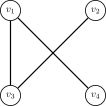
\includegraphics[width=\linewidth]{./fig/graph-example01.svg}
\end{image}%
\tcblower
\end{figureptx}%
\begin{figureptx}{A second graph.}{x:figure:fig-graph-example02}{}%
\begin{image}{0.375}{0.25}{0.375}%
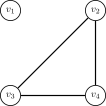
\includegraphics[width=\linewidth]{./fig/graph-example02.svg}
\end{image}%
\tcblower
\end{figureptx}%
\begin{figureptx}{A third graph.}{x:figure:fig-graph-example03}{}%
\begin{image}{0.375}{0.25}{0.375}%
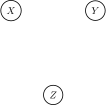
\includegraphics[width=\linewidth]{./fig/graph-example03.svg}
\end{image}%
\tcblower
\end{figureptx}%
\begin{figureptx}{A fourth graph.}{x:figure:fig-graph-example04}{}%
\begin{image}{0.375}{0.25}{0.375}%
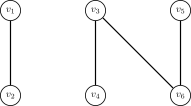
\includegraphics[width=\linewidth]{./fig/graph-example04.svg}
\end{image}%
\tcblower
\end{figureptx}%
\begin{figureptx}{A fifth graph.}{x:figure:fig-graph-example05}{}%
\begin{image}{0.375}{0.25}{0.375}%
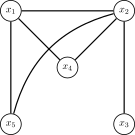
\includegraphics[width=\linewidth]{./fig/graph-example05.svg}
\end{image}%
\tcblower
\end{figureptx}%
\begin{figureptx}{A sixth graph (no, this is not a mistake).}{x:figure:fig-graph-example06}{}%
\begin{image}{0.375}{0.25}{0.375}%
\includegraphics[width=\linewidth]{./fig/graph-example06.svg}
\end{image}%
\tcblower
\end{figureptx}%
\end{exploration}%
\begin{exploration}{}{x:exploration:expl-graph-def-second-attempt}%
Below there are several examples of objects that are \emph{not} graphs. If necessary, modify your definition from \hyperref[x:exploration:expl-graph-def-first-attempt]{Problem~{\xreffont\ref{x:exploration:expl-graph-def-first-attempt}}}, and explain why the objects below do not meet your (possibly new) definition\textemdash{}but make sure the objects in \hyperref[x:exploration:expl-graph-def-first-attempt]{Problem~{\xreffont\ref{x:exploration:expl-graph-def-first-attempt}}} still do!%
\begin{figureptx}{Not a graph.}{x:figure:fig-graph-nonexample01}{}%
\begin{image}{0.375}{0.25}{0.375}%
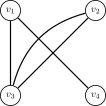
\includegraphics[width=\linewidth]{./fig/graph-nonexample01.svg}
\end{image}%
\tcblower
\end{figureptx}%
\begin{figureptx}{Not a graph.}{x:figure:fig-graph-nonexample02}{}%
\begin{image}{0.375}{0.25}{0.375}%
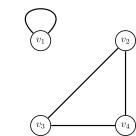
\includegraphics[width=\linewidth]{./fig/graph-nonexample02.svg}
\end{image}%
\tcblower
\end{figureptx}%
\begin{figureptx}{(Still) Not a graph.}{x:figure:fig-graph-nonexample03}{}%
\begin{image}{0.375}{0.25}{0.375}%
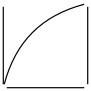
\includegraphics[width=\linewidth]{./fig/graph-nonexample03.svg}
\end{image}%
\tcblower
\end{figureptx}%
\end{exploration}%
\begin{definition}{}{x:definition:def-graph}%
\index{graph}%
A \terminology{graph} is ....%
\end{definition}
\begin{activity}{}{g:activity:idp105545028434832}%
Given the definition of a graph that we've come up with, exhibit two additional examples of a graph, as well as two non-examples.%
\end{activity}%
\end{sectionptx}
\end{chapterptx}
%
%
\typeout{************************************************}
\typeout{Chapter 3 Proof Techniques}
\typeout{************************************************}
%
\begin{chapterptx}{Proof Techniques}{}{Proof Techniques}{}{}{x:chapter:chap-proof-techniques}
%
%
\typeout{************************************************}
\typeout{Section 3.1 Direct Proof}
\typeout{************************************************}
%
\begin{sectionptx}{Direct Proof}{}{Direct Proof}{}{}{x:section:sec-direct-proof}
\begin{assemblage}{Guiding Questions.}{g:assemblage:idp105545028443536}%
In this section, we'll seek to answer the questions: %
\begin{itemize}[label=\textbullet]
\item{}What is a proof?%
\item{}What is a direct proof?%
\item{}What are some ideas for getting started\slash{}unstuck when stuck on a proof?%
\end{itemize}
%
\end{assemblage}
\end{sectionptx}
%
%
\typeout{************************************************}
\typeout{Section 3.2 Proof by Contradiction}
\typeout{************************************************}
%
\begin{sectionptx}{Proof by Contradiction}{}{Proof by Contradiction}{}{}{x:section:sec-contradiction}
\end{sectionptx}
%
%
\typeout{************************************************}
\typeout{Section 3.3 Proof via Contrapositive}
\typeout{************************************************}
%
\begin{sectionptx}{Proof via Contrapositive}{}{Proof via Contrapositive}{}{}{x:section:sec-contrapositive}
\end{sectionptx}
%
%
\typeout{************************************************}
\typeout{Section 3.4 Induction}
\typeout{************************************************}
%
\begin{sectionptx}{Induction}{}{Induction}{}{}{x:section:sec-induction}
\end{sectionptx}
\end{chapterptx}
%
%
\typeout{************************************************}
\typeout{Chapter 4 Set Theory}
\typeout{************************************************}
%
\begin{chapterptx}{Set Theory}{}{Set Theory}{}{}{x:chapter:chap-set-theory}
%
%
\typeout{************************************************}
\typeout{Section 4.1 The idea of a set}
\typeout{************************************************}
%
\begin{sectionptx}{The idea of a set}{}{The idea of a set}{}{}{x:section:sec-idea-of-sets}
\end{sectionptx}
%
%
\typeout{************************************************}
\typeout{Section 4.2 Operations with Sets}
\typeout{************************************************}
%
\begin{sectionptx}{Operations with Sets}{}{Operations with Sets}{}{}{x:section:sec-set-operations}
\end{sectionptx}
%
%
\typeout{************************************************}
\typeout{Section 4.3 Families of Sets}
\typeout{************************************************}
%
\begin{sectionptx}{Families of Sets}{}{Families of Sets}{}{}{x:section:sec-familes-of-sets}
\end{sectionptx}
\end{chapterptx}
%
%
\typeout{************************************************}
\typeout{Chapter 5 Functions}
\typeout{************************************************}
%
\begin{chapterptx}{Functions}{}{Functions}{}{}{x:chapter:chap-functions}
%
%
\typeout{************************************************}
\typeout{Section 5.1 Introduction to Functions}
\typeout{************************************************}
%
\begin{sectionptx}{Introduction to Functions}{}{Introduction to Functions}{}{}{x:section:sec-intro-to-functions}
\end{sectionptx}
%
%
\typeout{************************************************}
\typeout{Section 5.2 Properties of Functions}
\typeout{************************************************}
%
\begin{sectionptx}{Properties of Functions}{}{Properties of Functions}{}{}{x:section:sec-properties-of-functions}
\end{sectionptx}
\end{chapterptx}
%
%
\typeout{************************************************}
\typeout{Chapter 6 Further Explorations in Graph Theory}
\typeout{************************************************}
%
\begin{chapterptx}{Further Explorations in Graph Theory}{}{Further Explorations in Graph Theory}{}{}{x:chapter:chap-more-graphs}
%
%
\typeout{************************************************}
\typeout{Section 6.1 Trees and Cycles}
\typeout{************************************************}
%
\begin{sectionptx}{Trees and Cycles}{}{Trees and Cycles}{}{}{x:section:sec-trees-cycles}
\end{sectionptx}
%
%
\typeout{************************************************}
\typeout{Section 6.2 Graph Isomorphisms}
\typeout{************************************************}
%
\begin{sectionptx}{Graph Isomorphisms}{}{Graph Isomorphisms}{}{}{x:section:sec-graph-isomorphisms}
\end{sectionptx}
%
%
\typeout{************************************************}
\typeout{Section 6.3 Graph Invariants}
\typeout{************************************************}
%
\begin{sectionptx}{Graph Invariants}{}{Graph Invariants}{}{}{x:section:sec-graph-invariants}
\end{sectionptx}
\end{chapterptx}
%
\appendix%
%
\clearpage\phantomsection%
\addcontentsline{toc}{part}{Appendices}%
%
%
\typeout{************************************************}
\typeout{Appendix A On Mathematical Writing}
\typeout{************************************************}
%
\begin{appendixptx}{On Mathematical Writing}{}{On Mathematical Writing}{}{}{x:appendix:appendix-writing}
\end{appendixptx}
%
\backmatter%
%
\clearpage\phantomsection%
\addcontentsline{toc}{part}{Back Matter}%
%
%% The index is here, setup is all in preamble
%% Index locators are cross-references, so same font here
{\xreffont\printindex}
%
\end{document}